\documentclass[a4paper]{article}  

\usepackage{mathtools}
\usepackage{amsthm}
\usepackage{tikz}
\usepackage{algpseudocode}

\title{CS270 Homework 1}
\author{Valkyrie Savage}

\begin{document}
\maketitle

\begin{enumerate}
\item Routing and Fractional Flow
	\begin{enumerate}
	\item Following is a simple example of a graph in which the maximum congestion in optimal solutions to the path routing problem and the fractional flow problem differ, with the solution to the \textbf{path routing} on the left and the solution to the \textbf{fractional flow} on the right.
		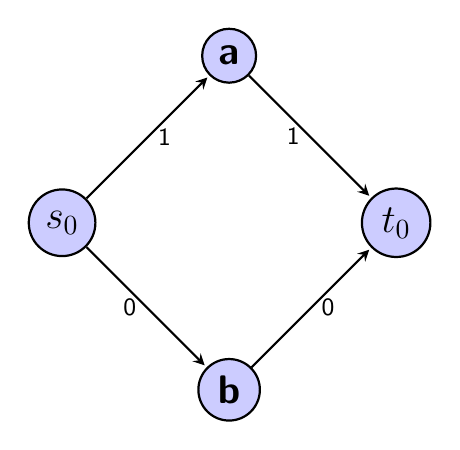
\begin{tikzpicture}[->,>=stealth,shorten >=1pt,auto,node distance=3cm,
 		thick,main node/.style={circle,fill=blue!20,draw,font=\sffamily\Large\bfseries}]

  		\node[main node] (B) {a};
  		\node[main node] (A) [below left of=B] {$s_0$};
  		\node[main node] (C) [below right of=A] {b};
  		\node[main node] (D) [below right of=B] {$t_0$};

  		\path[every node/.style={font=\sffamily\small}]
    		(B) edge node [left] {1} (D)
    		(A) edge node [right] {1} (B)
        		edge node [left]  {0} (C)
    		(C) edge node [right] {0} (D);
		\end{tikzpicture}
		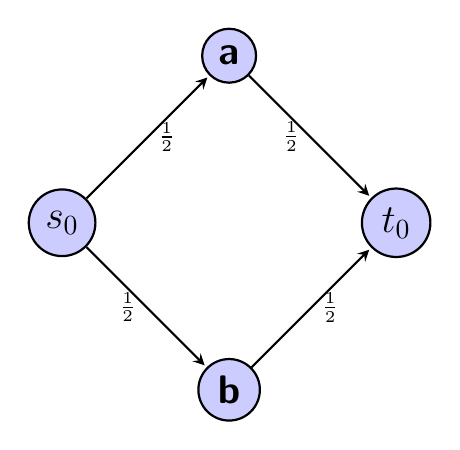
\begin{tikzpicture}[->,>=stealth,shorten >=1pt,auto,node distance=3cm,
 		thick,main node/.style={circle,fill=blue!20,draw,font=\sffamily\Large\bfseries}]

  		\node[main node] (B) {a};
  		\node[main node] (A) [below left of=B] {$s_0$};
  		\node[main node] (C) [below right of=A] {b};
  		\node[main node] (D) [below right of=B] {$t_0$};

  		\path[every node/.style={font=\sffamily\small}]
    		(B) edge node [left] {$\frac{1}{2}$} (D)
    		(A) edge node [right] {$\frac{1}{2}$} (B)
        		edge node [left]  {$\frac{1}{2}$} (C)
    		(C) edge node [right] {$\frac{1}{2}$} (D);
		\end{tikzpicture}\\
	\item Write out 206 of 264 except less than.
	\end{enumerate}
\item Equilibrium - pondered and completed but not written up as per instructions.
\item Maximum weight matching vs. minimum weight vertex cover
	\begin{enumerate}
	\item Hi, an algorithm
	\begin{algorithmic}
	\State $i \gets 3$
	\end{algorithmic}
	\item Hi, an analysis of the above
	\end{enumerate}
\end{enumerate}
\end{document}